\subsection{\texorpdfstring{SYSTEM OF TYPE \(E_{6}\)}{SYSTEM OF TYPE E\_6}}

\begin{enumerate}
\def\labelenumi{(\Roman{enumi})}
\tightlist
\item
  and (II) Let \(E = R^{8}\) , and let \(R_{8}\) be the root system in E constructed in no. 10. Let V be the vector subspace of E generated by the roots \(\alpha_{1}, \ldots, \alpha_{6}\) of \(R_{8}\) ; this is the orthogonal complement of the plane generated by the last two fundamental weights \(\omega = \varepsilon_{7} + \varepsilon_{8}\) and \(\pi = \varepsilon_{6} + \varepsilon_{7} + 2\varepsilon_{8}\) of \(R_{8}\) .
\end{enumerate}

Let \(R = R_{8} \cap V\) . This is a reduced root system with basis \((\alpha_{1}, \ldots, \alpha_{6})\) , and hence of type \(E_{6}\) . Its elements are:

\[
\begin{array}{c} \pm \varepsilon_ {i} \pm \varepsilon_ {j} (1 \leqslant i <   j \leqslant 5), \\ \pm \frac {1}{2} (\varepsilon_ {8} - \varepsilon_ {7} - \varepsilon_ {6} + \sum_ {i = 1} ^ {5} (- 1) ^ {\nu (i)} \varepsilon_ {i}) \text {with} \sum_ {i = 1} ^ {5} \nu (i) \text {even.} \end{array}
\]

The number of roots is \(n = \binom{5}{2}.4 + 2^5 = 72\) . The positive roots are

\[
\pm \varepsilon_ {i} + \varepsilon_ {j} (1 \leqslant i <   j \leqslant 5),
\]

\[
\frac {1}{2} \left(\varepsilon_ {8} - \varepsilon_ {7} - \varepsilon_ {6} + \sum_ {i = 1} ^ {5} (- 1) ^ {\nu (i)} \varepsilon_ {i}\right) \text {with} \sum_ {i = 1} ^ {5} \nu (i) \text {even}.
\]

\begin{enumerate}
\def\labelenumi{(\Roman{enumi})}
\setcounter{enumi}{2}
\item
  We have \(h = \frac{n}{6} = 12\) .
\item
  Let
\end{enumerate}

\[
\begin{array}{r l} \tilde {\alpha} & = \frac {1}{2} (\varepsilon_ {1} + \varepsilon_ {2} + \varepsilon_ {3} + \varepsilon_ {4} + \varepsilon_ {5} - \varepsilon_ {6} - \varepsilon_ {7} + \varepsilon_ {8}) \\ & = \alpha_ {1} + 2 \alpha_ {2} + 2 \alpha_ {3} + 3 \alpha_ {4} + 2 \alpha_ {5} + \alpha_ {6}, \end{array}
\]

which is a root. The sum of its coordinates with respect to \((\alpha_{i})\) is 11 = h - 1, so \(\tilde{\alpha}\) is the highest root. It is orthogonal to \(\alpha_{1}, \alpha_{3}, \alpha_{4}, \alpha_{5}, \alpha_{6}\) , and \((\tilde{\alpha}|\alpha_{2}) = 1\) . The completed Dynkin graph is

\pandocbounded{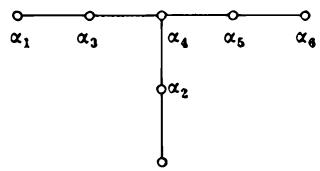
\includegraphics[keepaspectratio]{images/part002_9f0044a9.jpg}}

\begin{enumerate}
\def\labelenumi{(\Alph{enumi})}
\setcounter{enumi}{21}
\tightlist
\item
  Since \((\alpha |\alpha) = 2\) for all \(\alpha \in \mathbb{R}\) , we have \(\mathbb{R}^{\sim} = \mathbb{R}\) . For \(\Phi_{\mathbb{R}}\) , the squared length of the roots is \(\frac{1}{12}\) , so
\end{enumerate}

\[
\Phi_ {\mathrm{R}} (x, y) = (x | y) / 24, \quad \text { and } \quad \gamma (\mathrm{R}) = 144.
\]

\begin{enumerate}
\def\labelenumi{(\Roman{enumi})}
\setcounter{enumi}{5}
\tightlist
\item
  Calculating the fundamental weights gives:
\end{enumerate}

\[
\begin{array}{l} \omega_ {1} = \frac {2}{3} (\varepsilon_ {8} - \varepsilon_ {7} - \varepsilon_ {6}) = \frac {1}{3} (4 \alpha_ {1} + 3 \alpha_ {2} + 5 \alpha_ {3} + 6 \alpha_ {4} + 4 \alpha_ {5} + 2 \alpha_ {6}) \\ \omega_ {2} = \frac {1}{2} (\varepsilon_ {1} + \varepsilon_ {2} + \varepsilon_ {3} + \varepsilon_ {4} + \varepsilon_ {5} - \varepsilon_ {6} - \varepsilon_ {7} + \varepsilon_ {8}) \\ \quad = \alpha_ {1} + 2 \alpha_ {2} + 2 \alpha_ {3} + 3 \alpha_ {4} + 2 \alpha_ {5} + \alpha_ {6} = \tilde {\alpha} \\ \omega_ {3} = \frac {5}{6} (\varepsilon_ {8} - \varepsilon_ {7} - \varepsilon_ {6}) + \frac {1}{2} (- \varepsilon_ {1} + \varepsilon_ {2} + \varepsilon_ {3} + \varepsilon_ {4} + \varepsilon_ {5}) \\ \quad = \frac {1}{3} (5 \alpha_ {1} + 6 \alpha_ {2} + 10 \alpha_ {3} + 12 \alpha_ {4} + 8 \alpha_ {5} + 4 \alpha_ {6}) \\ \omega_ {4} = \varepsilon_ {3} + \varepsilon_ {4} + \varepsilon_ {5} - \varepsilon_ {6} - \varepsilon_ {7} + \varepsilon_ {8} \\ \quad = 2 \alpha_ {1} + 3 \alpha_ {2} + 4 \alpha_ {3} + 6 \alpha_ {4} + 4 \alpha_ {5} + 2 \alpha_ {6} \\ \omega_ {5} = \frac {2}{3} (\varepsilon_ {8} - \varepsilon_ {7} - \varepsilon_ {6}) + \varepsilon_ {4} + \varepsilon_ {5} \\ \quad = \frac {1}{3} (4 \alpha_ {1} + 6 \alpha_ {2} + 8 \alpha_ {3} + 12 \alpha_ {4} + 10 \alpha_ {5} + 5 \alpha_ {6}) \\ \omega_ {6} = \frac {1}{3} (\varepsilon_ {8} - \varepsilon_ {7} - \varepsilon_ {6}) + \varepsilon_ {5} \\ \quad = \frac {1}{3} (2 \alpha_ {1} + 3 \alpha_ {2} + 4 \alpha_ {3} + 6 \alpha_ {4} + 5 \alpha_ {5} + 4 \alpha_ {6}). \end{array}
\]

\begin{enumerate}
\def\labelenumi{(\Roman{enumi})}
\setcounter{enumi}{6}
\tightlist
\item
  Half the sum of the positive roots is \(\sum_{i=1}^{6} \omega_i\) , so
\end{enumerate}

\[
\begin{array}{r l} \rho & = \varepsilon_ {2} + 2 \varepsilon_ {3} + 3 \varepsilon_ {4} + 4 \varepsilon_ {5} + 4 (\varepsilon_ {8} - \varepsilon_ {7} - \varepsilon_ {6}) \\ & = 8 \alpha_ {1} + 11 \alpha_ {2} + 15 \alpha_ {3} + 21 \alpha_ {4} + 15 \alpha_ {5} + 8 \alpha_ {6}. \end{array}
\]

\begin{enumerate}
\def\labelenumi{(\Roman{enumi})}
\setcounter{enumi}{7}
\tightlist
\item
  By no. 10 (VIII) and § 1, no. 10, Prop. 28,
\end{enumerate}

\[
\mathrm{Q} (\mathrm{R}) = \mathrm{Q} (\mathrm{R} _ {8}) \cap \mathrm{V} = \mathrm{L} _ {3} \cap \mathrm{V} \quad \text { and } \quad \mathrm{P} (\mathrm{R}) = p (\mathrm{P} (\mathrm{R} _ {8})) = p (\mathrm{L} _ {3}),
\]

where p denotes the orthogonal projection of E onto V. We have

\[
p (\alpha_ {7}) = \alpha_ {7} - \frac {2}{3} \pi + \omega , \quad p (\alpha_ {8}) = \alpha_ {8} + \pi - 2 \omega .
\]

The group \(Q(R)\) has basis \((\alpha_{1},\ldots,\alpha_{6})\) . The group \(P(R)\) is generated by \(Q(R)\) and \(p(\alpha_{7})\) , since \(p(\alpha_{8})\in P(R_{8})\cap V=Q(R_{8})\cap V=Q(R)\) . We have \(3p(\alpha_{7})\in Q(R)\) and \(p(\alpha_{7})\notin Q(R)\) . Hence, the group \(P(R)/Q(R)\) is isomorphic to Z/3Z; it is generated, for example, by the image of \(\omega_{6}\) .

The connection index is 3.

\begin{enumerate}
\def\labelenumi{(\Roman{enumi})}
\setcounter{enumi}{8}
\tightlist
\item
  (IX) and (X) By § 2. no. 4. Prop. 7, the order of the Weyl group is 6!1.2.2.3.2.1.3 = \(2^{7}.3^{4}.5\) . The sequence of exponents has 6 terms between 1 and 11, and contains the integers 1, 5, 7, 11 which are coprime to 12. The other exponents \(m, m'\) are integers such that
\end{enumerate}

\[
m + m ^ {\prime} = 12.
\]

\[
(m + 1) \left(m ^ {\prime} + 1\right) (1 + 1) (5 + 1) (7 + 1) (11 + 1) = 2 ^ {7}. 3 ^ {4}. 5,
\]

in view of Chap. V. § 6, no. 2, formula (2) and Cor. 1 of Prop. 3. The second relation gives \((m + 1)(m' + 1) = 45\) , and since \(m + m' + 2 = 14\) , we obtain \(m = 4\) , \(m' = 8\) . Hence, the sequence of exponents is

\[
1, 4, 5, 7, 8, 11.
\]

\begin{enumerate}
\def\labelenumi{(\Roman{enumi})}
\setcounter{enumi}{10}
\tightlist
\item
  (XI) and (XII) Since the roots all have the same length, the automorphisms of the Dynkin graph are those of the underlying graph. Apart from the identity, there is only the automorphism \(\varepsilon\) which transforms \(\alpha_{1},\alpha_{3},\alpha_{4},\alpha_{5},\alpha_{6},\) \(\alpha_{2}\) into \(\alpha_{6},\alpha_{5},\alpha_{4},\alpha_{3},\alpha_{1},\alpha_{2}\) , respectively. Hence, \(\mathrm{A(R) / W(R)}\) is isomorphic to \(\mathbf{Z} / 2\mathbf{Z}\) ; since \(-1\in \mathrm{W(R)}\) (Chap. V. §6, no. 2, Cor. 3 of Prop. 3), \(\mathrm{A(R)}\) is isomorphic to \(\mathrm{W(R)}\times \{1, - 1\}\) and \(w_0\) can be identified with \(-\varepsilon\) . It follows that the non-identity element of \(\mathrm{A(R) / W(R)}\) defines the automorphism \(x\mapsto -x\) of \(\mathrm{P(R^{\prime}) / Q(R^{\prime})}\) .
\end{enumerate}

Moreover, \(P(R^{-})/Q(R^{-})\) has two non-identity elements of order 3. They define the two automorphisms of order 3 of the completed Dynkin graph.

